\documentclass[a4paper,titlepage]{ltjsarticle}
\usepackage{graphicx, color, xcolor}
\usepackage{ascmac}
\usepackage{float}
\usepackage{enumitem}
\usepackage{tabularray}
\usepackage{listings}
\usepackage{amssymb}
\usepackage{wrapfig}
\usepackage{diagbox}
\usepackage{siunitx}
\usepackage{enshuc}

\lstset{
    basicstyle=\ttfamily,
    frame=single,
    breaklines=true,
    numbers=left,
    numberstyle=\tiny,
    stepnumber=1,
    numbersep=5pt,
    tabsize=2,
    captionpos=b,
    keywordstyle=\color{blue},
    commentstyle=\color{green!60!black},
    stringstyle=\color{red},
    showstringspaces=false,
    language=VHDL
}

\renewcommand{\thesubsubsection}{・}

\title{情報科学演習C\\課題1}
\author{植村 向陽}
\affiliation{ソフトウェア科学コース}
\studentid{09B24008}
\date{提出日:\today}
\begin{document}
\maketitle

\section{課題1-1}
\subsection*{1. \texttt{ping}コマンドについて}
\subsubsection{pingコマンド}        
\verb|ping|コマンドは引数で与えられた接続先にICMPエコーリクエストを継続的に送信し，接続先からの応答を受信することで，接続先にデータを送る際の遅延，パケットロス率，接続先のIPアドレスなどを確認するためのコマンドである．
\subsubsection{実行結果}
\begin{verbatim}
$ ping exp001
\end{verbatim}
を実行したところ，以下図 \ref{ping} のような結果が表示された．
\begin{figure}[H]
    \centering
    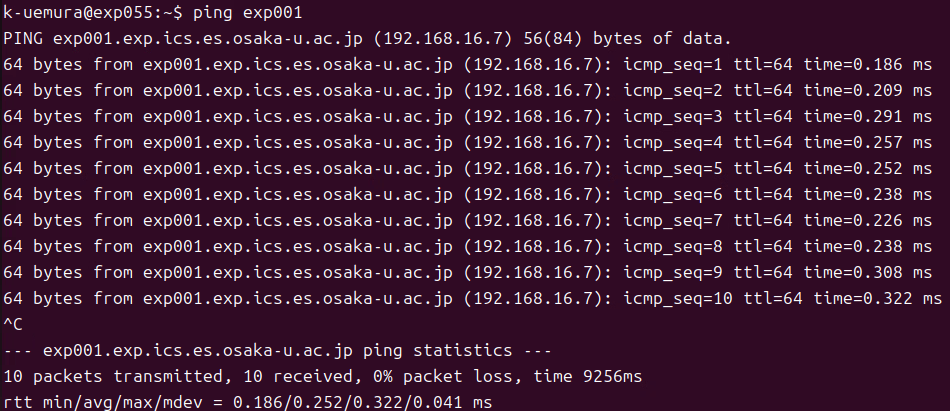
\includegraphics[scale = 0.6]{ping10.png}
    \caption{pingコマンドの実行結果}
    \label{ping}
\end{figure}
\subsubsection{考察}
実行結果より\verb|exp001|のIPアドレスは\verb|192.168.16.7|であることがわかる．また，\verb|time=|の後の値が応答時間であり，最後の行の表示から平均応答時間は0.252msであることがわかる．またすべてのパケットが応答を受け取っているため，パケットロス率は0\%であることがわかる．
\subsection*{2. ウェブブラウザの挙動}
\verb|https://www.osaka-u.ac.jp/ |と \verb| https://133.1.138.1/ |をブラウザで開いたところ
どちらも大阪大学のトップページが表示された．そのため二つのアドレスは同じものを指していることがわかる．

\subsection*{3. \texttt{nslookup}コマンドについて}
\verb|nslookup|コマンドはホスト名をIPアドレスに変換するか，その逆を行うためのコマンドである．このコマンドを\verb|exp001|と\verb|www.osaka-u.ac.jp|を引数として実行したところそれぞれ以下図 \ref{nslookup1}， \ref{nslookup2}のような結果が得られた．
\begin{figure}[H]
    \centering
    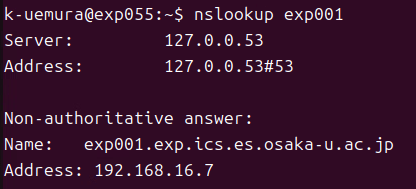
\includegraphics[scale = 0.8]{nslookup1.png}
    \caption{nslookupコマンドの実行結果1}
    \label{nslookup1}
\end{figure}
\begin{figure}[H]
    \centering
    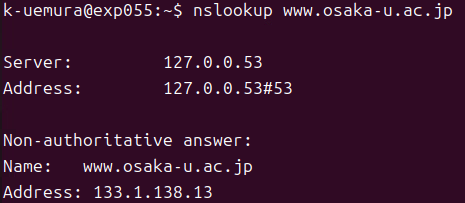
\includegraphics[scale = 0.8]{nslookup2.png}
    \caption{nslookupコマンドの実行結果2}
    \label{nslookup2}
\end{figure}
この実行結果からホスト名\verb|exp001|のIPアドレスは\verb|192.168.16.7|,ホスト名\verb|www.osaka-u.ac.jp|のIPアドレスは\verb|133.1.138.1|であることがわかる．
\section{課題1-2}
\subsection*{4. \texttt{/usr/sbin/arp -a}コマンドについて}
\subsubsection{実行結果}
\verb|ip neigh|はIPアドレスとMACアドレスの対応を表示するコマンドである．このコマンドを実行したところ以下図 \ref{ipneigh} のような結果が得られた．
\begin{figure}[H]
    \centering
    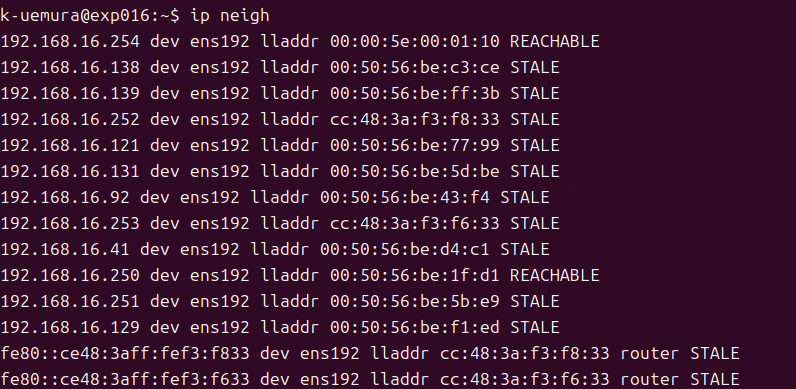
\includegraphics[scale = 0.7]{ipneigh.png}
    \caption{ip neighコマンドの実行結果}
    \label{ipneigh}
\end{figure}
そして各行において一番最初の項目がIPアドレス，\verb|lladdr|の後の項目が対応するMACアドレスであり，最後の項目はそのIPアドレスがどのような状態であるかを表している．\verb|REACHABLE|の場合はそのIPアドレスが現在到達可能であることを表しており，\verb|STALE|の場合はそのIPアドレスが現在到達可能かどうかわからないことを表している．
\subsection*{5. \texttt{ping}と\texttt{/usr/sbin/arp -a}の関係}
\verb|exp024|,\verb|exp041|, \verb|exp084|に対して\verb|ping|コマンドを実行したところそれぞれ以下図 \ref{ping24} \ref{ping41} \ref{ping84} のような結果が得られた．
\begin{figure}[H]
    \centering
    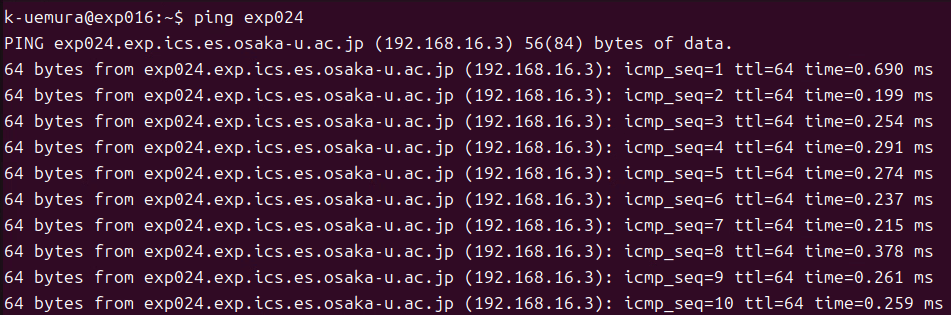
\includegraphics[scale = 0.6]{ping24.png}
    \caption{exp024に対するpingコマンドの実行結果}
    \label{ping24}
\end{figure}
\begin{figure}[H]
    \centering
    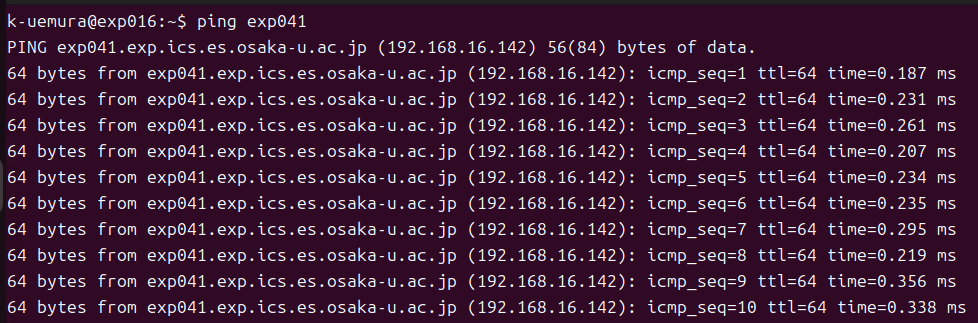
\includegraphics[scale = 0.6]{ping41.png}
    \caption{exp041に対するpingコマンドの実行結果}
    \label{ping41}
\end{figure}
\begin{figure}[H]
    \centering
    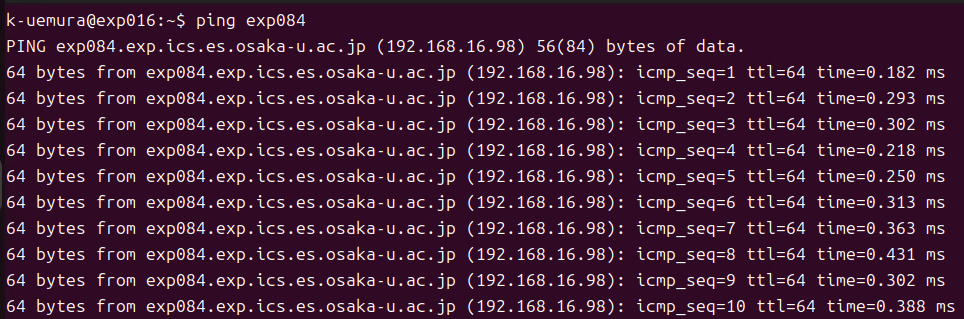
\includegraphics[scale = 0.6]{ping84.png}
    \caption{exp084に対するpingコマンドの実行結果}
    \label{ping84}
\end{figure}
これにより\verb|exp024|のIPアドレスは\verb|192.168.16.3|, \verb|exp041|のIPアドレスは\verb|192.168.16.142|, \verb|exp084|のIPアドレスは\verb|192.168.16.98|であることがわかる．
さらにこの後\verb|ip neigh|コマンドを実行したところ以下図 \ref{ipneigh2} のような結果が得られた．
\begin{figure}[H]
    \centering
    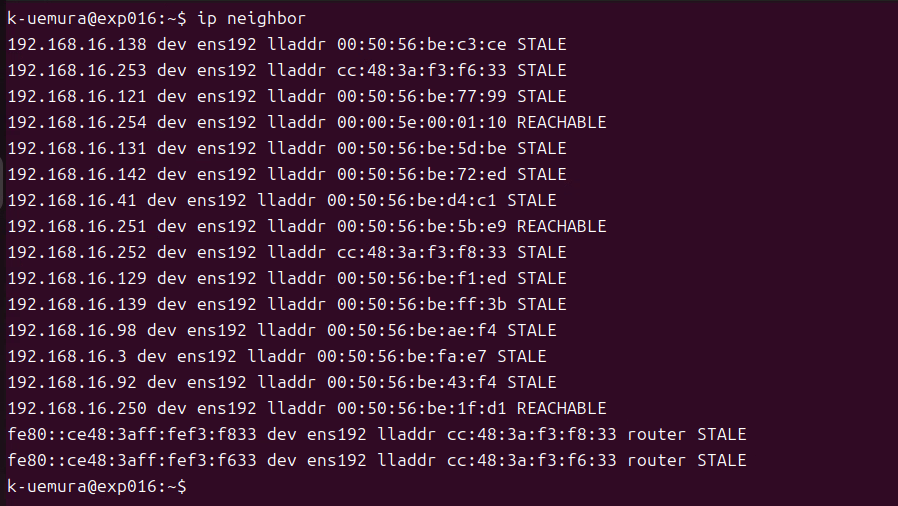
\includegraphics[scale = 0.6]{ipneigh2.png}
    \caption{ip neighコマンドの実行結果}
    \label{ipneigh2}
\end{figure}
最初に行った\verb|ip neigh|のIPアドレスに加えて，pingを実行した\verb|exp024|,\verb|exp041|, \verb|exp084|のIPアドレスも表示されていることがわかる．
\subsubsection{考察}
このような結果になったのは\verb|ping|で通信を行った際にそのIPアドレスとMACアドレスの対応が\verb|arp|プロトコルによって調べられ，その履歴が保存されたためだと考えられる．

\subsection*{6. \texttt{/usr/sbin/tracepath}について}
\subsubsection{実行結果}
前の課題で\verb|ping|を実行した\verb|exp024|,\verb|exp041|, \verb|exp084|に対して\verb|tracepath|コマンドを実行したところそれぞれ以下図 \ref{trace24} \ref{trace41} \ref{trace84} のような結果が得られた．
\begin{figure}[H]
    \centering
    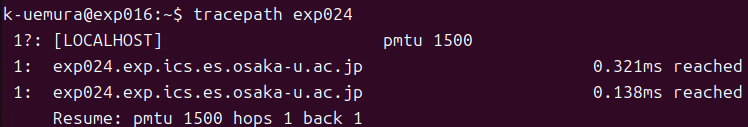
\includegraphics[scale = 0.7]{trace24.png}
    \caption{exp024に対するtracepathコマンドの実行結果}
    \label{trace24}
\end{figure}
\begin{figure}[H]
    \centering
    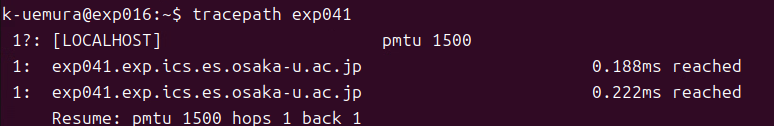
\includegraphics[scale = 0.7]{trace41.png}
    \caption{exp041に対するtracepathコマンドの実行結果}
    \label{trace41}
\end{figure}
\begin{figure}[H]
    \centering
    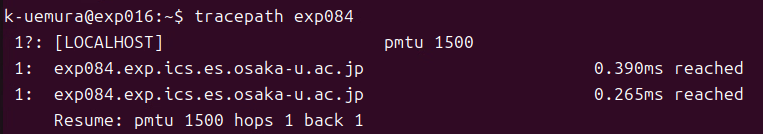
\includegraphics[scale = 0.7]{trace84.png}
    \caption{exp084に対するtracepathコマンドの実行結果}
    \label{trace84}
\end{figure}
一方，\verb|www.ics.es.osaka-u.ac.jp|，\verb|icsintgw.ics.es.osaka-u.ac.jp|に対しても同様に\verb|tracepath|コマンドを実行したところそれぞれ以下図 \ref{traceweb} \ref{traceintgw} のような結果が得られた．
\begin{figure}[H]
    \centering
    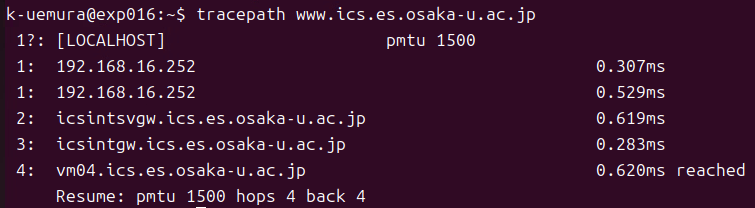
\includegraphics[scale = 0.7]{traceweb.png}
    \caption{www.ics.es.osaka-u.ac.jpに対するtracepathコマンドの実行結果}
    \label{traceweb}
\end{figure}
\begin{figure}[H]
    \centering
    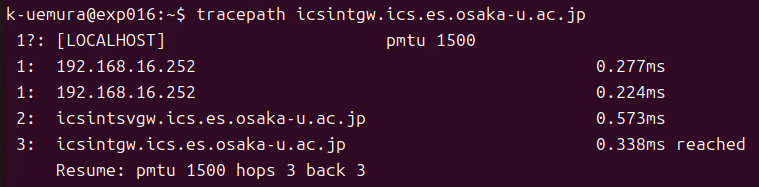
\includegraphics[scale = 0.7]{traceintgw.png}
    \caption{icsintgw.ics.es.osaka-u.ac.jpに対するtracepathコマンドの実行結果}
    \label{traceintgw}
\end{figure}
最初に\verb|tracepath|を実行した\verb|exp024|,\verb|exp041|, \verb|exp084|はゲートウェイを経由せずに直接通信が行われているのに対して，\verb|www.ics.es.osaka-u.ac.jp|はゲートウェイ\verb|icsintgw.ics.es.osaka-u.ac.jp|を経由して通信が行われていることがわかる．
\subsubsection{考察}
以上の結果から\verb|exp024|,\verb|exp041|, \verb|exp084|は同じネットワーク内に存在しているのに対して，\verb|www.ics.es.osaka-u.ac.jp|はゲートウェイ\verb|icsintgw.ics.es.osaka-u.ac.jp|を挟んで異なるネットワークに存在していることがわかる．
\subsection*{7. 演習室のネットワーク構成の予想}
これまでの課題の結果から\verb|expXXX|はすべてゲートウェイ\verb|icsintgw.ics.es.osaka-u.ac.jp|の内側のネットワークに存在していると考えられる．一方，\verb|www.ics.es.osaka-u.ac.jp|はゲートウェイの外側に存在していることがわかる．
\subsection*{8. \texttt{/bin/netstat -r}について}
\verb|ip route|を実行したところ以下図 \ref{iproute} のような結果が得られた．
\begin{figure}[H]
    \centering
    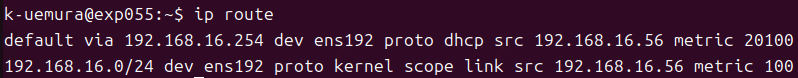
\includegraphics[scale = 0.7]{iproute.png}
    \caption{ip routeコマンドの実行結果}
    \label{iproute}
\end{figure}
1行目の実行結果の意味は以下のようになる．
\begin{itemize}
    \item \verb|default|\\
    外のネットワークに出ていくすべての通信を表している．
    \item \verb|via 192.168.16.254|\\
    \verb|default|の通信はすべてこのIPアドレスを持つゲートウェイを経由して行われることを表している．
    このipアドレスは\verb|icsintgw.ics.es.osaka-u.ac.jp|の仮想アドレスである(演習資料より)．
    \item \verb|dev ens192|\\
    このルートは\verb|dev ens192|という名前のインターフェースを使用して行われることを表している．
    \item \verb|proto dhcp|\\
    このルートはプロトコルDHCPによって設定されたことを表している．
    \item \verb|src 192.168.16.56|\\
    このルートを使用する際の送信元IPアドレス，すなわちこのPCのIPアドレスは\verb|192.168.16.56|であることを表している．
    \item \verb|metric 20100|\\
    ルートの優先度を表している．この値が小さいほど優先される．
\end{itemize}
そして2行目の実行結果の意味は以下のようになる．
\begin{itemize}
    \item \verb|192.168.16.0/24|\\
    このネットワーク内のすべてのIPアドレスを表している．
    \item \verb|dev ens192|\\
    1行目と同様
    \item \verb|proto kernel|\\
    このルートはカーネル(OS)によって設定されたことを表している．
    \item \verb|scope link|\\
    \verb|link|スコープのルートであることを表している．このルートは同じネットワーク内の通信に使用される．
    \item \verb|src 192.168.16.56|\\
    1行目と同様
    \item \verb|metric 100|\\
    1行目と同様
\end{itemize}
この結果から\verb|expXXX|はすべて同じネットワーク内に存在しており，\verb|www.ics.es.osaka-u.ac.jp|はゲートウェイを経由して通信が行われていることから，このPCは\verb|www.ics.es.osaka-u.ac.jp|とは異なるネットワークに存在していることがわかる．つまり前の課題で述べたネットワーク構成は正しいことがわかる．
\subsection*{9. ARPの仕組み}
\subsubsection{実行結果}
先ほどの課題の操作から約30分後に\verb|ip neigh|コマンドを実行したところ以下図 \ref{ipneigh3} のような結果が得られた．
\begin{figure}[H]
    \centering
    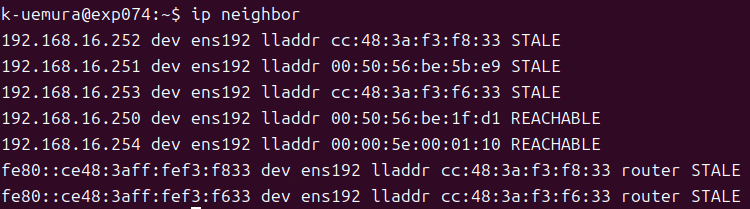
\includegraphics[scale = 0.7]{ipneigh3.png}
    \caption{ip neighコマンドの実行結果}
    \label{ipneigh3}
\end{figure}
先ほどの\verb|ipneigh|の結果から\verb|exp024|,\verb|exp041|, \verb|exp084|のIPアドレスを含む複数のIPアドレスが消えているのがわかる．
\subsubsection{考察}
このような結果になったのは\verb|ip neigh|コマンドで表示されるIPアドレスとMACアドレスの対応の履歴は一定時間が経過すると消えるようになっているためだと考えられる．
\section{課題1-3}
\subsection*{10. C言語の標準ライブラリ関数とシステムコールの違い}
システムコールはカーネルの機能を呼び出し，特権モードで動作する．そのため使用しているOSに強く依存し，使用した場合プログラムの互換性が失われる可能性がある．一方，ライブラリ関数はユーザーモードで動作し，システムコールを呼び出すこともあるが，OSに依存しないように内部で実装されているため，使用してもプログラムの互換性が失われる可能性は低い．
さらに，システムコールは呼び出すたびにカーネルモードとユーザーモードの切り替えが必要であるため，ライブラリ関数を使用するよりもオーバーヘッドが大きい．そのため実行速度が下がる可能性がある．一方，ライブラリ関数はユーザーモードで動作し，システムコールを呼び出す回数が少ないように実装されているため，システムコールを直接使用するよりもオーバーヘッドが小さい．そのため実行速度が上がる可能性がある．
しかし，システムコールを直接使用することで，より細かい制御が可能になるため，特定の状況ではシステムコールを直接使用することが有利な場合もある．
\subsection*{11. \texttt{strace}について}
\verb|strace -c echo hello|を実行したところ以下図 \ref{straceecho} のような結果が得られた．
\begin{figure}[H]
    \centering
    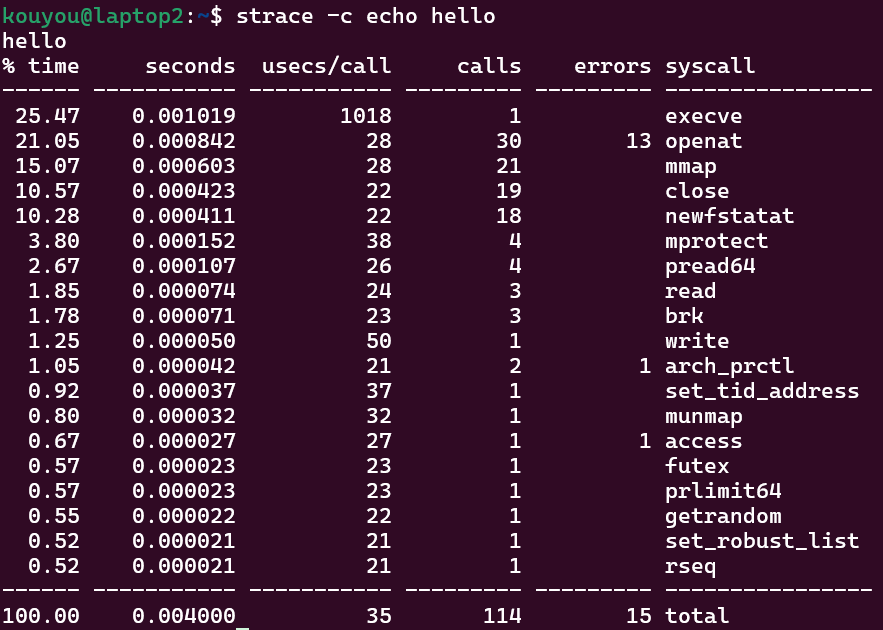
\includegraphics[scale = 0.5]{straceecho.png}
    \caption{strace -c echo helloの実行結果}
    \label{straceecho}
\end{figure}
各行について説明すると，\verb|% time|はそのシステムコールが全体の実行時間のうちどれくらいの割合を占めているかを表している．\verb|seconds|はそのシステムコールが実行されるのにかかった時間を表している．\verb|usecs/call|はそのシステムコールが1回呼び出されるのにかかった平均時間を表している．\verb|calls|はそのシステムコールが何回呼び出されたかを表している．\verb|errors|はそのシステムコールが呼び出された際にエラーが発生した回数を表している．最後の列はシステムコールの名前である．
この結果から\verb|echo hello|を実行する際には\verb|execve|システムコールが最も多く呼び出されていることがわかる．このシステムコールは子プロセスを生成する際に使用されるシステムコールである．
また，\verb|strace -c cat hoge|を実行したところ以下図 \ref{stracecat} のような結果が得られた．
\begin{figure}[H]
    \centering
    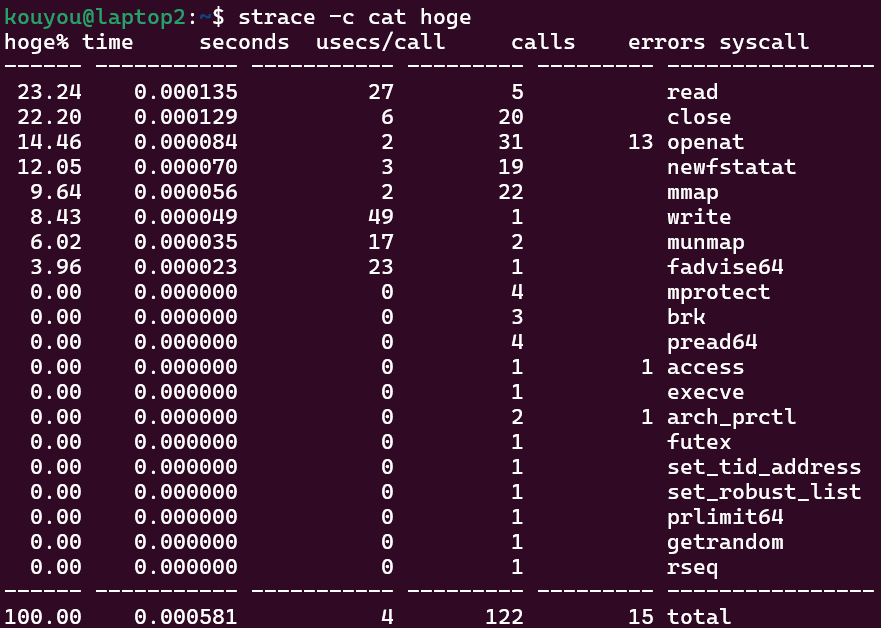
\includegraphics[scale = 0.5]{stracecat.png}
    \caption{strace -c cat hogeの実行結果}
    \label{stracecat}
\end{figure}
この結果から\verb|cat hoge|を実行する際には\verb|read|システムコールが最も多く呼び出されていることがわかる．このシステムコールはファイルからデータを読み取る際に使用されるシステムコールである．

\section{発展課題}
\subsection*{1. 各種ネットワーク関連コマンドについて}
\subsubsection{telnetコマンド}
\verb|telnet|コマンドは\verb|telnet|プロトコルを使用するホストと通信を行うためのコマンドである．このコマンドを実行したところ以下図 \ref{telnet} のようにコマンドの入力を促す表示がされた．
\begin{figure}[H]
    \centering
    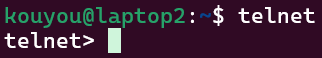
\includegraphics[scale = 1.2]{telnet.png}
    \caption{telnetコマンドの実行結果}
    \label{telnet}
\end{figure}
\subsubsection{sshコマンド}
\verb|ssh|コマンドは\verb|ssh|プロトコルと呼ばれる暗号化プロトコルを用いて通信する際に使用される.
\verb|ssh|コマンドを用いて\verb|github|に接続したところ以下図\ref{ssh}のようになった.
\begin{figure}[H]
    \centering
    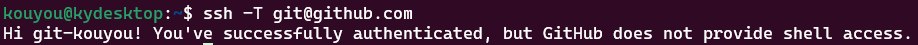
\includegraphics[scale = 0.6]{ssh.png}
    \caption{sshコマンドの実行結果}
    \label{ssh}
\end{figure}
\subsection*{2. \texttt{strace}の挙動の違い}
まず，図 \ref{hello0} のようにコードをコメントアウトして\verb|strace|を実行したところ，図 \ref{stracehello0} のような結果が得られた．
\begin{figure}[H]
    \begin{verbatim}
    ...
    char message[] = "hello";
    //char message[] = "hello\n";
    ...
    fwrite(message, strlen(message), 1,stdout);
    //write(0, message, strlen(message));
    ...
    \end{verbatim}
    \caption{コードのコメントアウト1}
    \label{hello0}
\end{figure}
\begin{figure}[H]
    \centering
    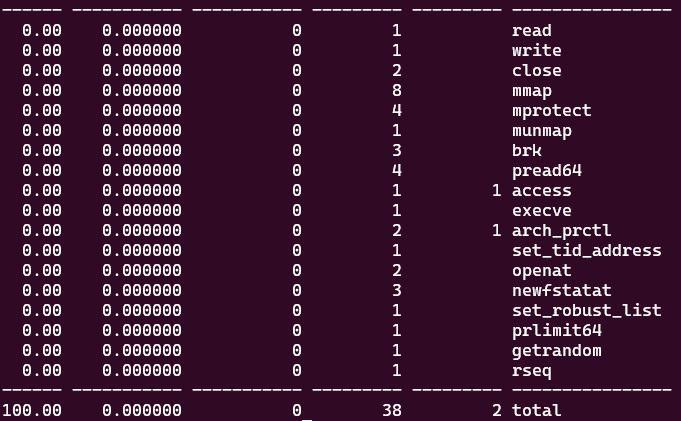
\includegraphics[scale = 0.65]{hello0.png}
    \caption{straceの実行結果1}
    \label{stracehello0}
\end{figure}
次に図 \ref{hello1} のようにコードをコメントアウトして\verb|strace|を実行したところ，以下図 \ref{stracehello1} のような結果が得られた．
\begin{figure}[H]
    \begin{verbatim}
    ...
    char message[] = "hello";
    //char message[] = "hello\n";
    ...
    //fwrite(message, strlen(message), 1,stdout);
    write(0, message, strlen(message));
    ...
    \end{verbatim}
    \caption{コードのコメントアウト2}
    \label{hello1}
\end{figure}
\begin{figure}[H]
    \centering
    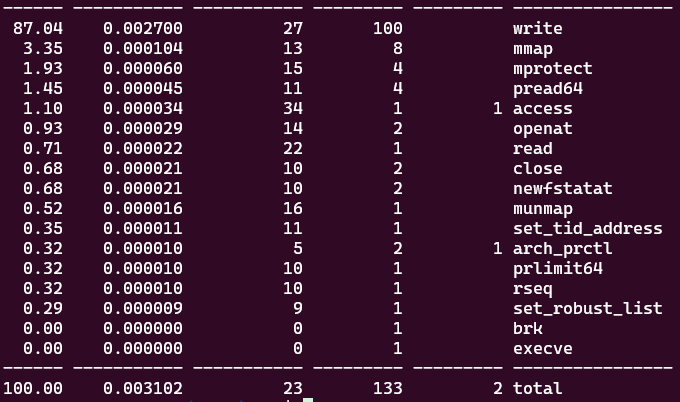
\includegraphics[scale = 0.65]{hello1.png}
    \caption{straceの実行結果2}
    \label{stracehello1}
\end{figure}
さらに今度は図 \ref{hello2} のようにコードをコメントアウトして\verb|strace|を実行したところ，以下図 \ref{stracehello2} のような結果が得られた．
\begin{figure}[H]
    \begin{verbatim}
    ...
    //char message[] = "hello";
    char message[] = "hello\n";
    ...
    fwrite(message, strlen(message), 1,stdout);
    //write(0, message, strlen(message));
    ...
    \end{verbatim}
    \caption{コードのコメントアウト3}
    \label{hello2}
\end{figure}
\begin{figure}[H]
    \centering
    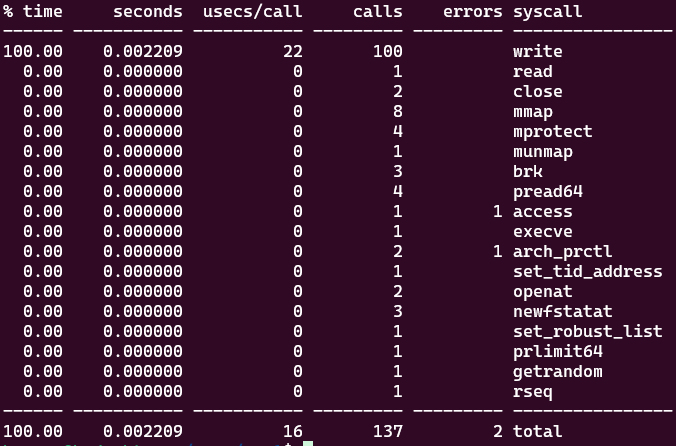
\includegraphics[scale = 0.65]{hello2.png}
    \caption{straceの実行結果3}
    \label{stracehello2}
\end{figure}
最後に図 \ref{hello3} のようにコードをコメントアウトして\verb|strace|を実行したところ，以下図 \ref{stracehello3} のような結果が得られた．
\begin{figure}[H]
    \begin{verbatim}
    ...
    //char message[] = "hello";
    char message[] = "hello\n";
    ...
    //fwrite(message, strlen(message), 1,stdout);
    write(0, message, strlen(message));
    ...
    \end{verbatim}
    \caption{コードのコメントアウト4}
    \label{hello3}
\end{figure}
\begin{figure}[H]
    \centering
    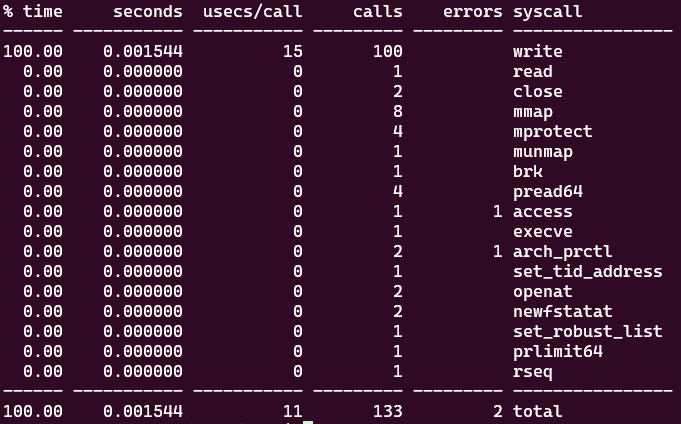
\includegraphics[scale = 0.65]{hello3.png}
    \caption{straceの実行結果4}
    \label{stracehello3}
\end{figure}
\subsubsection{考察}
この実行結果から改行を含まない文字列のときは\verb|fwrite|関数を使用した場合は\verb|write|システムコールを直接使用した場合より圧倒的にシステムコールの呼び出し回数が少ないことが分かる.一方，改行を含む文字列のときは\verb|fwrite|関数を使用した場合も\verb|write|システムコールを直接使用した場合も同じ回数だけシステムコールが呼び出されていることが分かる．
このような結果になったのは\verb|fwrite|関数は改行を含まない文字列を出力する際にはバッファリングを行い，複数回の出力がまとめられて一度にシステムコールが呼び出されるためだと考えられる．一方，改行が含まれる場合，改行自体を出力するのにシステムコールを使用するため，文字列の1回の出力のたびにシステムコールが呼び出されるためこのような結果になったと考えられる．
\section{感想，意見，疑問等}
今回ネットワークに関する様々な\verb|linux|コマンドを扱ったがあまりネットワークに対する知識がなく，各コマンドの動作や意味を理解するのに苦労した.
\end{document}